\chapter{El proyecto de un vistazo}

\section{El problema}

Cuando una persona se pierde en un bosque, encontrarla pronto puede salvarle la vida. Un dron con
cámara recorre en minutos lo que a una brigada a pie le tomaría horas, y lo hace sin arriesgar a
nadie. Pero desde el aire una persona ocupa unos pocos píxeles, las copas de los árboles la tapan, la
luz cambia y el viento mueve al dron. Para que el dron sirva hay que resolver tres preguntas:
\begin{enumerate}
  \item \textbf{¿Hay alguien en la imagen?} (percepción: detector de personas);
  \item \textbf{¿Dónde está en el mapa, y qué tan seguro estoy?} (estimación: localización en el
        terreno y fusión de observaciones);
  \item \textbf{¿Cómo recorro el bosque sin perder a nadie?} (control y misión).
\end{enumerate}

\section{Qué hace la simulación}

\begin{itemize}
  \item \textbf{Bosque por factores:} se genera un bosque con tres niveles de cobertura de copas (15,
        45 y 75~\%), dos condiciones de luz (sol alto o sombras largas), con o sin viento, y de una a
        tres personas de pie, sentadas o acostadas en lugares al azar.
  \item \textbf{Dron:} un x500 de PX4 de 2.114~kg con una cámara de $1280\times960$ que mira hacia
        abajo, una IMU, GPS y un LiDAR.
  \item \textbf{Piloto:} PX4~1.17 o ArduCopter~4.7, en SITL (el mismo programa que volaría en el dron
        real).
  \item \textbf{Controlador:} la cascada del piloto automático o una red neuronal 15-64-32-4 que
        imita a la cascada y corre dentro de PX4 (módulo \emph{Neural Control}).
  \item \textbf{Detector:} YOLO26s ajustado con 3000 imágenes del simulador (AP50 = 0.954).
  \item \textbf{Localizador:} corta el rayo de cada detección con el suelo, calcula su elipse de error
        y fusiona las detecciones de una misma persona.
  \item \textbf{Misión:} barrido en franjas a 30~m, re-observación de candidatas dudosas, avisos GPS,
        aterrizaje y métricas (personas localizadas, falsas alarmas, error).
\end{itemize}

\section{Arquitectura}

\begin{figure}[H]
\centering
\begin{tikzpicture}[
  nodo/.style={draw,rounded corners,fill=#1,minimum width=3.1cm,minimum height=1cm,align=center,font=\small},
  nodo/.default=white,
  flecha/.style={-{Stealth[length=2.5mm]},thick},
  et/.style={font=\scriptsize\ttfamily,fill=white,inner sep=1pt}]
  \node[nodo=orange!15,minimum width=4.2cm,minimum height=2cm] (gz) at (0,0) {\textbf{Gazebo Harmonic}\\ bosque, x500, cámara,\\ LiDAR, viento};
  \node[nodo=red!10] (px4) at (6,0) {\textbf{PX4 SITL}\\ (o ArduCopter)\\ cascada o red neuronal};
  \node[nodo=black!5] (dds) at (6,-2.6) {agente\\ uXRCE-DDS};
  \node[nodo=black!5] (puente) at (0,-2.6) {\cod{ros_gz_bridge}};
  \node[nodo=blue!10] (det) at (-3.4,-5) {\cod{detector_node}\\ YOLO26s (GPU)};
  \node[nodo=green!12] (loc) at (1,-5) {\cod{localizador_node}\\ rayo--terreno y fusión};
  \node[nodo=green!12] (mis) at (6,-5) {\cod{mision_node}\\ barrido, avisos};
  \node[nodo=yellow!15] (gps) at (6,-7.3) {aviso GPS\\ \cod{/personas/*}};
  \node[nodo=black!5] (gcs) at (10.2,-2.6) {MAVProxy\\ consola y mapa};
  \draw[flecha] (gz) -- node[et,above]{motores, sensores} (px4);
  \draw[flecha] (px4) -- node[et,right]{odometría} (dds);
  \draw[flecha] (gz) -- (puente);
  \draw[flecha] (puente) -| node[et,pos=0.7]{/camera} (det);
  \draw[flecha] (det) -- node[et,above]{/detecciones} (loc);
  \draw[flecha] (dds) -| node[et,pos=0.75,left]{odometría} (loc);
  \draw[flecha] (loc) -- node[et,above]{/personas/candidatas} (mis);
  \draw[flecha] (mis) -- node[et,right]{consignas} (dds);
  \draw[flecha] (mis) -- (gps);
  \draw[flecha] (px4.east) -| node[et,pos=0.3,above]{MAVLink} (gcs);
\end{tikzpicture}
\caption{Programas y tópicos principales. La cadena es \emph{imagen $\rightarrow$ detección
$\rightarrow$ localización $\rightarrow$ fusión $\rightarrow$ decisión $\rightarrow$ consigna
$\rightarrow$ control}.}
\label{fig:arquitectura}
\end{figure}

\begin{figure}[H]
\centering
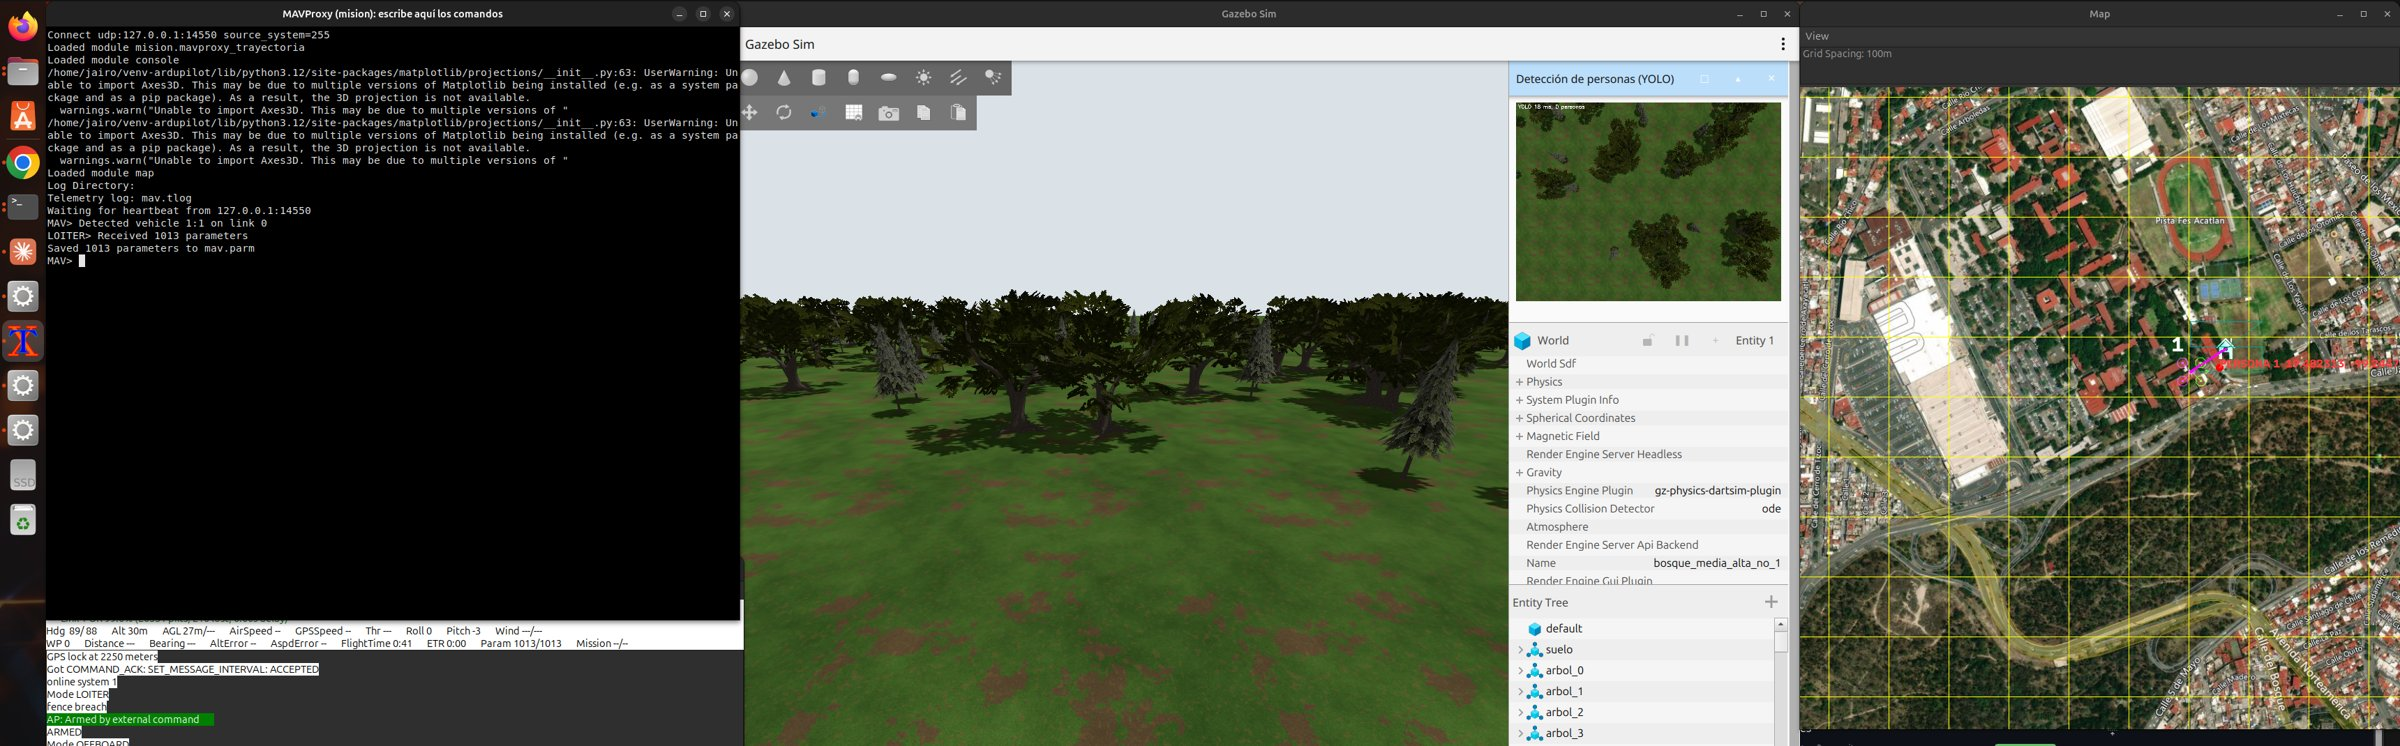
\includegraphics[width=\textwidth]{pantalla_mavproxy.jpg}
\caption{La simulación en marcha: a la izquierda la terminal y la consola de MAVProxy (la estación de
tierra), al centro Gazebo con el panel de detección, a la derecha el mapa con la persona 1 ya
localizada.}
\end{figure}

\section{Un vuelo completo}

\begin{figure}[H]
\centering
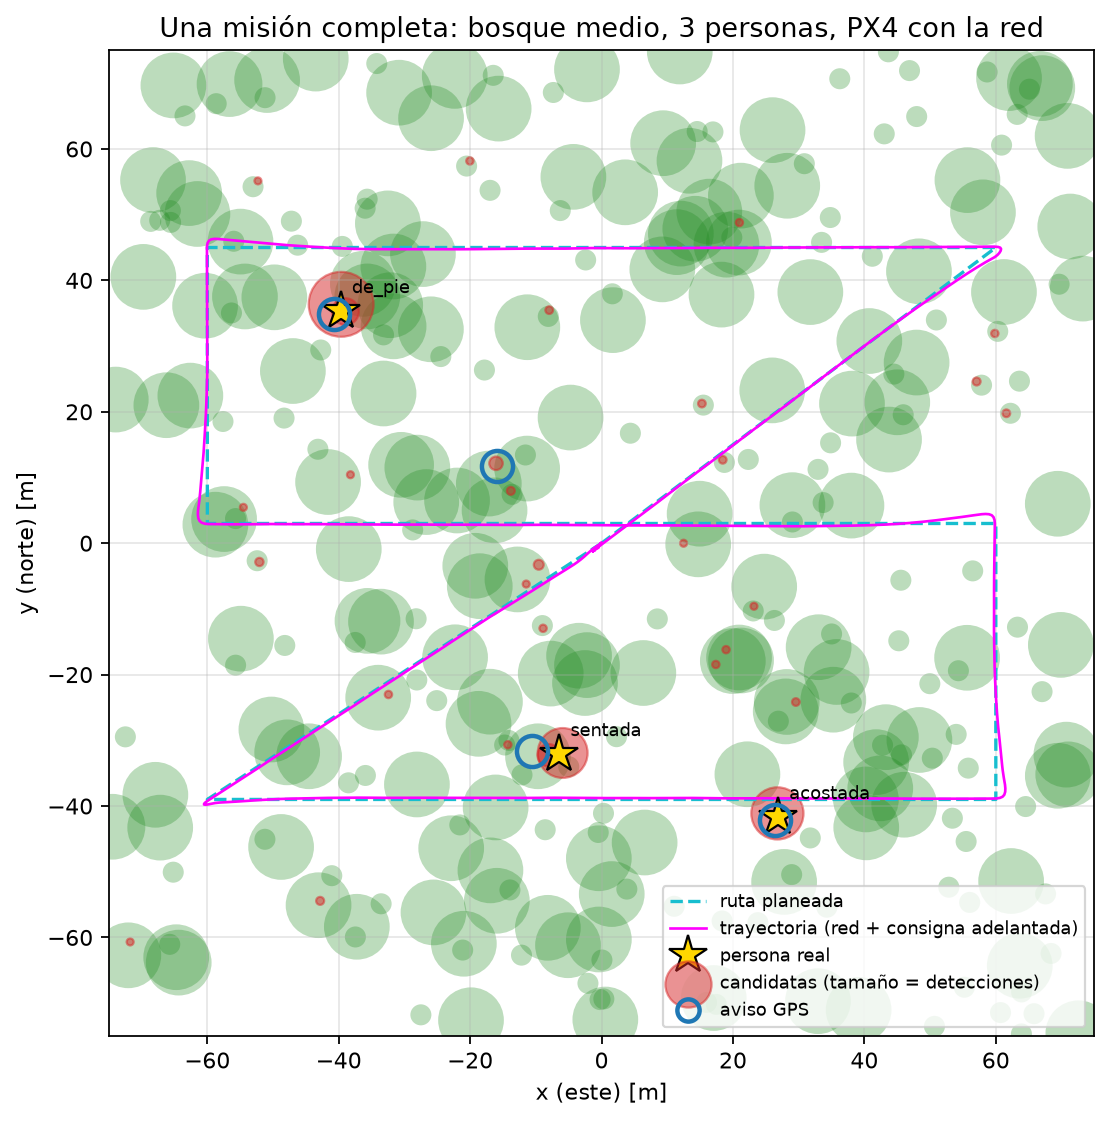
\includegraphics[width=0.85\textwidth]{mision_mapa.png}
\caption{Una misión real de la simulación, vista desde arriba: el bosque (círculos verdes), la ruta
planeada, lo que voló el dron, las candidatas que fue juntando el localizador, las tres personas
reales y los avisos GPS.}
\label{fig:mision-mapa}
\end{figure}

La figura~\ref{fig:mision-mapa} resume todo el libro: el dron sigue franjas paralelas, el detector ve
personas y también cosas que no lo son (puntos rojos), el localizador junta las detecciones de cada
lugar, y la misión avisa cuando una candidata ya está confirmada. Las tres personas se encontraron con
menos de 1~m de error; también hubo un aviso falso entre unos robles. Entender por qué pasa cada cosa
es el objetivo de las páginas que siguen.

\section{Convenciones de marcos}

\begin{itemize}
  \item \textbf{Mundo:} ENU (\emph{x} este, \emph{y} norte, \emph{z} arriba), en metros, con origen en
        el centro del bosque. PX4 y ArduPilot usan NED: $N=y$, $E=x$, $D=-z$.
  \item \textbf{Cuerpo:} en ROS FLU (\emph{x} al frente, \emph{y} a la izquierda, \emph{z} arriba); en
        PX4 FRD (\emph{y} a la derecha, \emph{z} abajo).
  \item El mundo está georreferenciado en 19.4826° N, 99.2447° O, 2250~m, así que el GPS del dron y
        los avisos dan coordenadas reales.
\end{itemize}
